\documentclass[12pt,a4paper,titlepage]{scrartcl}

\usepackage{comment}
\usepackage[main=english]{babel}
\usepackage[utf8]{inputenc}
\usepackage[T1]{fontenc}
\usepackage{lmodern}
\usepackage{geometry}
\geometry{left=2.5cm,right=2.5cm,top=2.5cm,bottom=3cm,head=29pt,foot=25pt}
\setlength{\footheight}{25pt}
\usepackage{microtype}
\usepackage{amsmath,amssymb,mathtools}
\numberwithin{equation}{section}
\numberwithin{table}{section}
\numberwithin{figure}{section}
\usepackage{siunitx}
\sisetup{locale=US, 
    separate-uncertainty=true, 
    per-mode=fraction,
    }
\usepackage{booktabs}
\usepackage{multirow}
\usepackage{graphicx}
\usepackage{float}
\usepackage{caption}
\usepackage{subcaption}
\usepackage[automark]{scrlayer-scrpage}
\usepackage[most]{tcolorbox}
\usepackage{hyperref}
\usepackage{pdfpages}
\usepackage{csvsimple-l3}
\usepackage{longtable}
\usepackage{graphicx}

%\input{../../jupyterpackages.tex}

% jupyter nbconvert --to latex 'Path'
% enferne usepackages und begin{document} und end{document}
% \input in main.tex mit \input{Path}


\newcommand{\pdfabbildung}[2]{%
    \refstepcounter{figure}%
    \addcontentsline{lof}{figure}{\protect\numberline{\thefigure}#1}%
    \label{#2}%
}

\newcommand{\pdftabelle}[2]{%
    \refstepcounter{table}%
    \addcontentsline{lot}{table}{\protect\numberline{\thetable}#1}%
    \label{#2}%
}


\hypersetup{colorlinks=true, linkcolor=blue!60!black, urlcolor=blue!60!black, citecolor=blue!60!black}

\clearpairofpagestyles

\chead{%
    \versuch\hfill\autor\\
    \rule{\textwidth}{0.2pt}%
}
\cfoot{%
    \rule{\textwidth}{0.2pt}\\[-0.5ex]
    \pagemark\ 
}
\addtokomafont{pagefoot}{\small}
\setlength{\parindent}{0pt}

\newtcolorbox{resultbox}[1][]{ 
    enhanced,
    colback=black!4!white,
    colframe=black!65!black,
    boxrule=0.8pt,
    arc=0.0mm,
    title=#1,
    fonttitle=\bfseries,
    %drop shadow
}


\newcommand{\versuch}{Experiment 15}
\newcommand{\titel}{Inclined Plane}
\newcommand{\praktikum}{Begginners Physics Lab 1}
\newcommand{\autor}{Jonathan Gießen}
\newcommand{\gruppe}{Group 8}
\newcommand{\datum}{15. September 2026}
\newcommand{\betreuer}{Matha Reece}

\begin{document}

\pagestyle{scrheadings}

\begin{titlepage}



    \centering
    \vspace*{4cm}
    {\large University of Heidelberg\par}
    {\small Faculty of Physics and Astronomy\par}
    {\Large \praktikum\par}
    \vspace{0.8cm}
    {\LARGE \bfseries \versuch\ -- \titel\par}
    \vspace{1.5cm}

    \begin{tabular}{ll}
        \textbf{Author:} & \autor\\
        \textbf{Group:} & \gruppe\\
        \textbf{Supervisor:} & \betreuer\\
        \textbf{Experiment Date:} & \datum\\
    \end{tabular}

    \vfill
    \hrulefill\
\end{titlepage}

\tableofcontents

\bigskip
\begin{tcolorbox}[colback=gray!5,colframe=gray!60,boxrule=0.8pt,arc=0.01mm,title=AI-Disclaimer]
    AI tools were used to assist in translating, as well as in the generation of text in section \ref{sec:Einleitung}
\end{tcolorbox}

\clearpage



\section{Introduction}\label{sec:Einleitung}
The experiment investigates the fundamental mechanics of rigid bodies moving down an inclined plane. By observing different rolling bodies specifically a solid cylinder and a hollow cylinder the experiment explores how mass distribution affects rotational and translational motion. The main objectives are to quantitatively determine the acceleration of these bodies as they roll down the ramp and to verify the law of conservation of mechanical energy by comparing the initial potential energy with the final translational and rotational kinetic energy.




\section{Basic Principles and theories}\label{sec:Grundlagen}
The motion of a round body rolling down an inclined plane without slipping is governed by both linear and rotational dynamics. Two primary physical frameworks are utilized to analyze this motion: Newton's laws of motion and the principle of energy conservation.

\subsection{Dynamics and Acceleration}
When a body rolls down an inclined plane with an angle $\varphi$, it experiences a downhill force component from gravity ($F_H = mg \sin\varphi$) and an opposing static friction force ($F_R$). This friction force exerts a torque (moment of force) $M$ relative to the center of mass, causing the body to rotate. The relationship between torque, the moment of inertia $I$, and angular acceleration $\frac{d\omega}{dt}$ is given by:
\begin{equation}
    M = F_R \cdot r = I \frac{d\omega}{dt}
\end{equation}
Using the rolling without slipping condition, the velocity of the center of gravity is $v_s = r\omega$. Differentiating this yields the relationship between linear acceleration $a_s$ and angular acceleration, allowing us to express the friction force as:
\begin{equation}
    F_R = \frac{I}{r^2} \cdot a_s
\end{equation}
Applying Newton's second law for linear motion along the plane ($m a_s = mg \sin\varphi - F_R$) and substituting the friction force, the linear acceleration of the rolling body is derived as:
\begin{equation}
    a_s = \frac{mg \sin\varphi}{m + \frac{I}{r^2}}\label{eq:acceleration_formula}
\end{equation}
This formula demonstrates that the acceleration depends on the body's moment of inertia, explaining why a hollow cylinder and a solid cylinder roll at different rates despite having the same radius.\cite{PAPskript}

\subsection{Conservation of Energy}
The motion can also be analyzed through the conservation of mechanical energy. Assuming no energy is lost to non-conservative forces (like air resistance or kinetic friction, since the static friction does no work), the initial potential energy is fully converted into kinetic energy. The total energy $W_{ges}$ is the sum of translational kinetic energy, rotational kinetic energy, and potential energy:
\begin{equation}
    W_{ges} = \frac{1}{2}mv^2 + \frac{1}{2}I\omega^2 + mgh
\end{equation}
As the body descends a vertical height $h$, the decrease in potential energy ($mgh$) equals the increase in total kinetic energy ($\frac{1}{2}mv^2 + \frac{1}{2}I\omega^2$).

\subsection{Gaussian error propagation}
The errors of the measured quantities are propagated using the Gaussian error propagation formula:
\begin{equation}
    \sigma_f = \sqrt{\sum_{i=1}^{N} \left(\frac{\partial f}{\partial x_i}\right)^2 \sigma_{x_i}^2}
\end{equation}

as well as the addition of statistical and systematic errors in quadrature:

\begin{equation}
    \sigma_{total} = \sqrt{\sigma_{stat}^2 + \sigma_{sys}^2}
\end{equation}



    
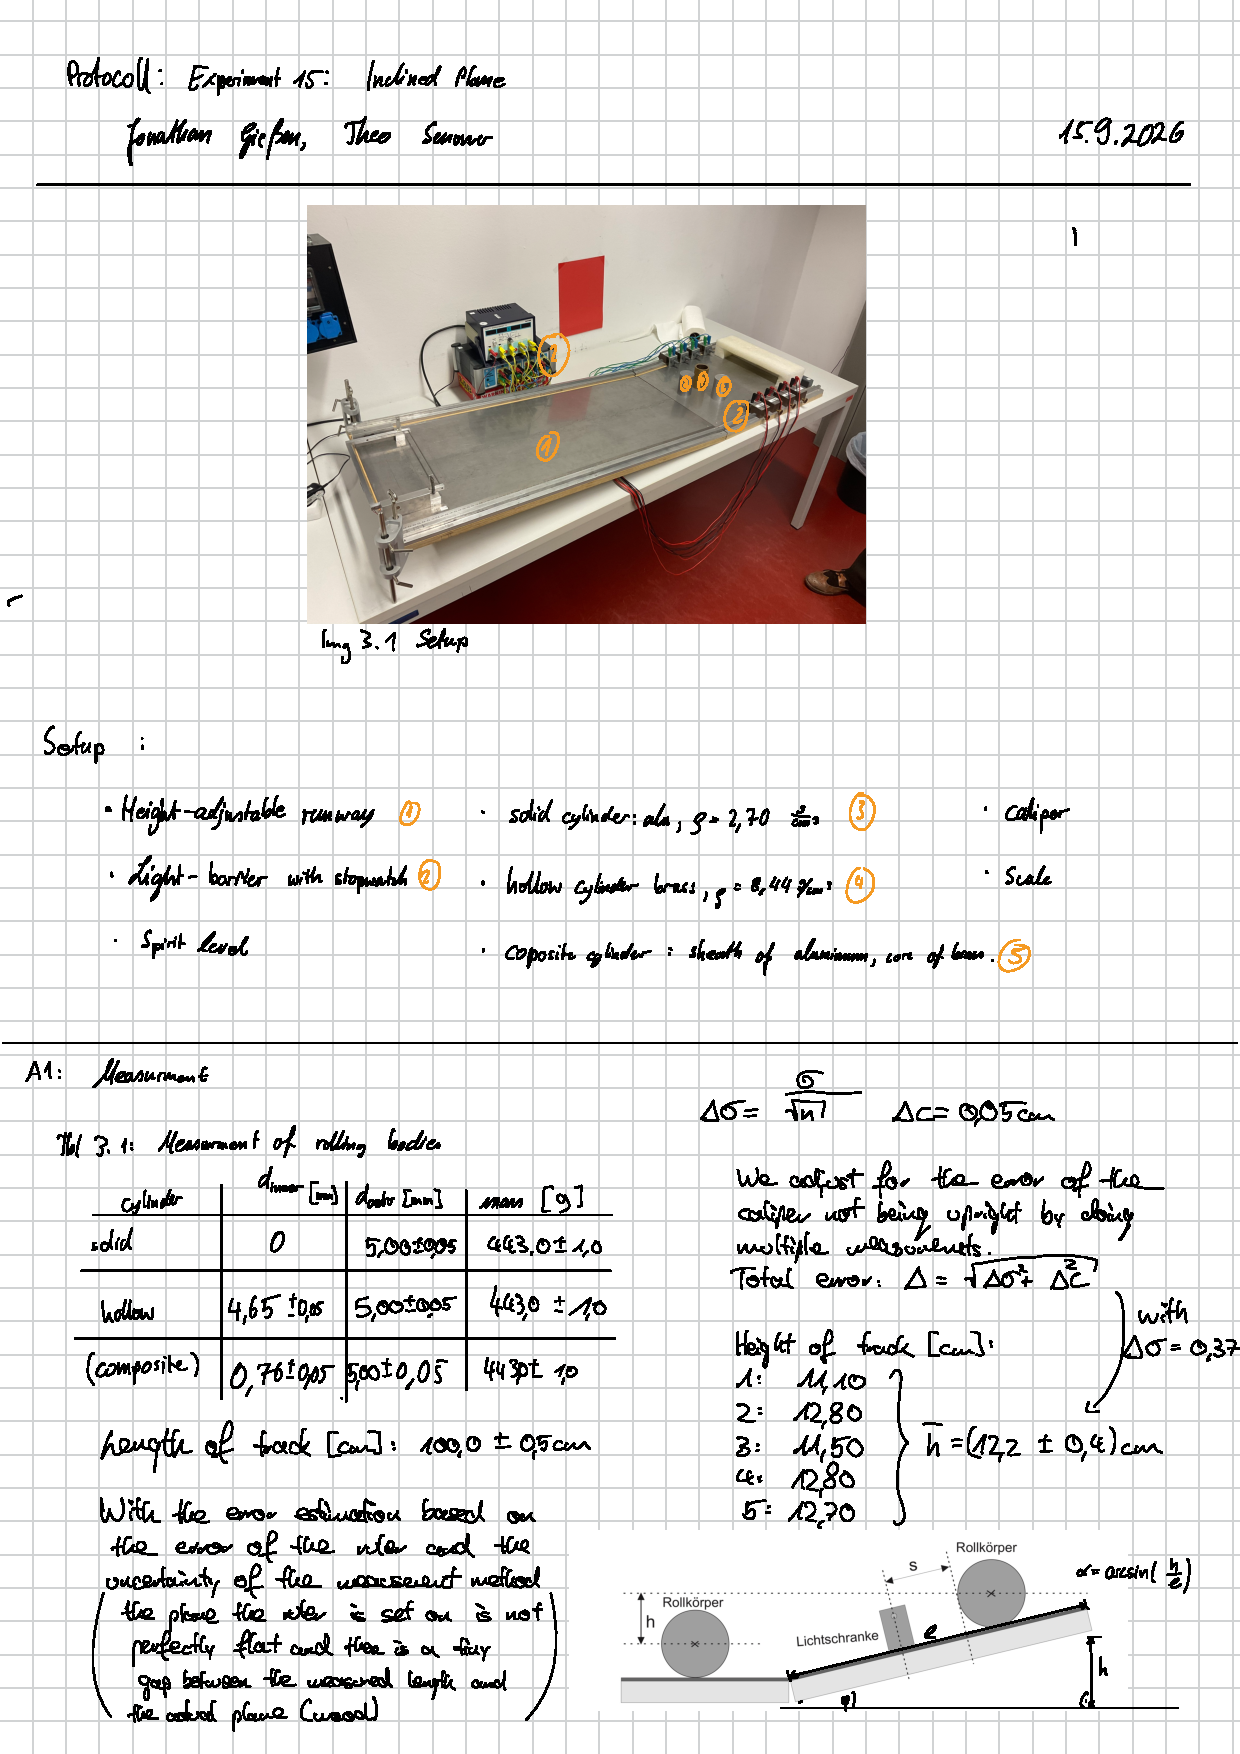
\includepdf[
    pages=-,
    width=\textwidth,
    height=0.95\textheight,
    keepaspectratio,
    pagecommand={\thispagestyle{scrheadings}},
    pagecommand*={\thispagestyle{scrheadings}\section{Measuring Protocol}\subsection{Setup and Tasks}}
]{../Messprotokoll 15.pdf}


\subsection{Execution of the Experiment}
The Experimental procedure involves the following main steps:

\begin{enumerate}
    \item \textbf{Setup and Geometry Measurement:} Familiarizing with the light barrier control unit and stopwatch system. Measuring the diameters of the test bodies (solid and hollow cylinders) using a caliper. Using a spirit level to ensure the inclined plane has an even inclination across its entire width, adjusting the supports if necessary (No adjustment was needed in this case).
    
    \item \textbf{Qualitative Analysis of Motion:} Verifing uniformly accelerated motion by placing the light barriers at appropriate intervals ($t \propto \sqrt{s}$). Observing and explain qualitatively why bodies with different mass distributions require different amounts of time to reach the bottom.
    
    \item \textbf{Quantitative Acceleration Measurement:} Place the light barriers along the incline and measure their exact distances $s$ from the starting mechanism. Release the solid and hollow cylinders and record the time it takes for them to pass the barriers. Repeat this measurement 5 times for each rolling body.
    
    \item \textbf{Energy Conservation Study:} To evaluate the conservation of energy, two light barriers are posiioned on the horizontal section at the end of the ramp. The final translational velocity of the bodies are measured. The calculated total kinetic energy will then be compared to the initial potential energy, which is derived from the height difference of the plane.
\end{enumerate}

\section{Evaluation}

\subsection{Exercise 1: Comparison of Acceleration (theoretical vs. experimental)}

The acceleration of the rolling bodies can be calculated using the derived formula:
\begin{equation}
    a_s = \frac{g \sin\varphi}{1 + \frac{I}{mr^2}}
\end{equation}     

The Moment of inertia $I$ for a solid cylinder is $I = \frac{1}{2}mr^2$, and for a hollow cylinder, it is $I = m(r_{out}^2 + r_{in}^2)$

With the measured parameters of the cylinders, the theoretical accelerations can be calculated. The parameters are summarized in Table \ref{tab:cylinder_parameters}.

\begin{table}[H]
    \centering
    \caption{Parameters of the cylinders used in the experiment.}
    \label{tab:cylinder_parameters}
    \begin{tabular}{l|c|c}
        \toprule
        \textbf{Parameter} & \textbf{Solid Cylinder} & \textbf{Hollow Cylinder} \\
        \midrule
        Mass [g] & \num{443.0(1.0)} & \num{443.0(1.0)} \\
        Inner diameter [m] & 0 & \num{46.5(0.05)e-3} \\
        Outer diameter [m] & \num{50.00(0.05)e-3} & \num{50.00(0.05)e-3} \\
        Moment of Inertia [\si{\kilo\gram\times\meter\squared}] & \num{1.384(4)e-4}  & \num{2.582(7)e-4} \\
        \bottomrule
    \end{tabular}
\end{table}

To calculate the theoretical acceleration, the angle of inclination $\varphi$ of the ramp is needed. This can be determined from the height difference $h$ and the length of the ramp $L$ using the relation:

\begin{equation}
    \sin\varphi = \frac{h}{L}
\end{equation}

\begin{figure}[H]
    \centering
    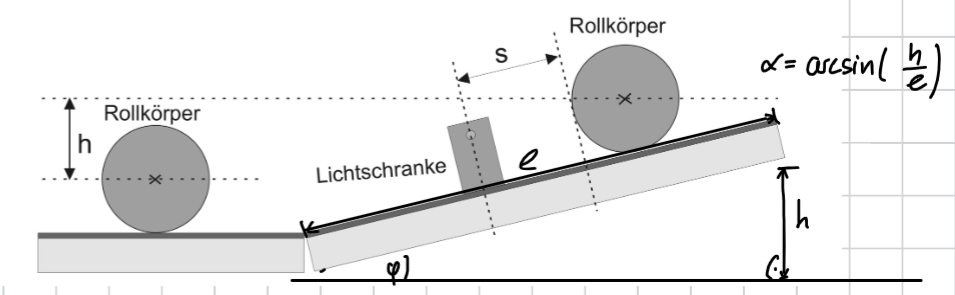
\includegraphics[width=0.7\textwidth]{img/inclined_plane_schematic.png}
    \caption{Schematic representation of the inclined plane with height $h$ and length $L$. \cite{PAPskript}}
    \label{fig:inclined_plane}
\end{figure}

with the measured height $h = \qty{12.2(4)e-2}{\text{m}}$ and the length of the track $l = \qty{1.000(5)}{\text{m}}$, the angle of inclination can be calculated as:
\begin{align}
    \varphi &= \arcsin\left(\frac{h}{L}\right) = \arcsin\left(\frac{\num{12.2(4)e-2}}{\num{1.000(5)}}\right) \\
    &\approx \num{7.01(24)}^\circ = \qty{0.122(4)}{\text{rad}}
\end{align}

Therefore, the theoretical accelerations for the solid and hollow cylinders can be calculated as (Equation \ref{eq:acceleration_formula}):
\begin{align}
    a_{solid} &= \frac{g \sin\varphi}{1 + \frac{I_{solid}}{m r^2}} = \qty{0.798(26)}{\meter\per\second\squared} \\
    a_{hollow} &= \frac{g \sin\varphi}{1 + \frac{I_{hollow}}{m r^2}} = \qty{0.619(21)}{\meter\per\second\squared}
\end{align}


Now, the experimentally determined times are plotted quadratically $t^2$ against the distance $s$. The slope of the linear fit corresponds to the acceleration, which can be compared to the theoretical values.

\begin{figure}[H]
    \centering
    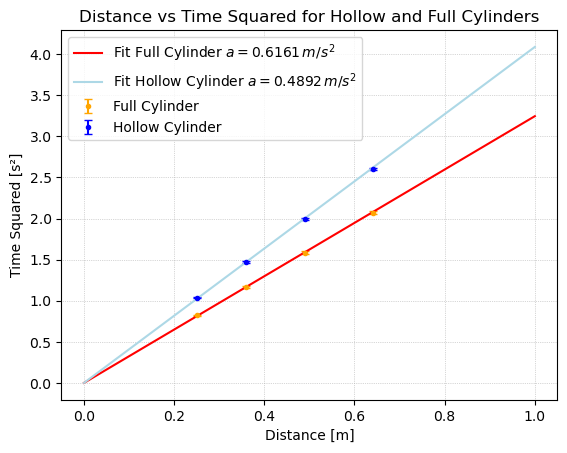
\includegraphics[width=0.8\textwidth]{img/E1.png}
    \caption{Comparison of theoretical and experimental accelerations for solid and hollow cylinders.}
    \label{fig:acceleration_comparison}
\end{figure}

The function used for the linear fit is $t^2 = \frac{2}{a} s$, where $a$ is the acceleration. The slope of the fit line gives the value of $\frac{2}{a}$.
The accelerations obtained from the fit are:
\begin{align}
    a_\text{solid, exp} &= \qty{0.6161(29)}{\meter\per\second\squared} \\
    a_\text{hollow, exp} &= \qty{0.4892(15)}{\meter\per\second\squared}
\end{align}
The experimental results show that the solid cylinder accelerates faster than the hollow cylinder, which is consistent with the theoretical predictions.

Interestingly, the experimental acceleration of both cylinders is much lower than the theoretical values.

The sigma-deviation of the experimental values from the theoretical ones can be calculated as:
\begin{align}
    \sigma_\text{solid} &= \frac{|a_\text{solid, exp} - a_\text{solid, theo}|}{\sigma_\text{hollow, theo}} \approx 6.65  \Rightarrow 6.7\sigma \\
    \sigma_\text{hollow} &= \frac{|a_\text{hollow, exp} - a_\text{hollow, theo}|}{\sigma_\text{solid, theo}} \approx 6.18 \Rightarrow 6.2\sigma
\end{align}

\begin{resultbox}[Conclusion]
    The experimental results for the accelerations of the solid and hollow cylinders show a significant deviation from the theoretical predictions, with both results being lower than expected. The calculated values are:
        \begin{center}
        \centering
        \begin{tabular}{lcc}
            \toprule
            \textbf{Value} & \textbf{Solid Cylinder} & \textbf{Hollow Cylinder} \\
            \midrule
            Theoretical Acceleration:& \num{0.798(26)} & \num{0.619(21)} \\
            Experimental Acceleration:& \num{0.6161(29)} & \num{0.4892(15)} \\
            \midrule
            Deviation: & \num{6.7} $\sigma$ & \num{6.2}$\sigma$ \\
            \bottomrule
            \end{tabular}
        \end{center}
\end{resultbox}

\subsection{Exercise 2: Calculating the kinetic Energy}

For calculatiung the kinetic energy, the final velocities of the cylinders are measured using two light barriers at the end of the ramp. The time taken to pass between the two barriers is recorded, and the velocity is calculated as:
\begin{equation}
    v = \frac{d}{t}
\end{equation}

Through the conservation of energy, the initial potential energy $E_{pot} = mgh$ should equal the total kinetic energy $E_{kin} = \frac{1}{2}mv^2 + \frac{1}{2}I\omega^2$. The rotational kinetic energy can be expressed in terms of the linear velocity using the rolling condition $\omega = \frac{v}{r}$.

The height difference equation can be derived from the geometry and the starting distance from the end of the ramp.

\begin{figure}
    \centering
    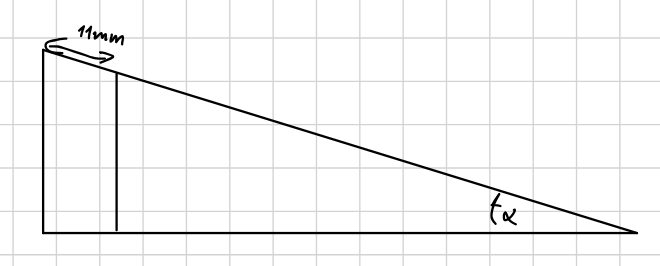
\includegraphics[width=0.7\textwidth]{img/height_calc.png}
    \caption{Schematic representation of the height difference $h$ and the length of the ramp $L$.}
    \label{fig:height_difference}
\end{figure}

For the height difference $h$, we can use the following relation (intercept theorem):

\begin{equation}
    h = \frac{h}{l} \cdot \left(l-11\si{\milli\meter}\right) = \qty{0.121(4)e-2}{\meter}
\end{equation}

The potential energy for the cylinders equals:
\begin{equation}
    E_{pot} = (\num{443(1)})\,\si{\gram} \cdot 9.81\,\si{\meter\per\second\squared} \cdot \qty{0.121(4)e-2}{\meter} = \qty{0.524(18)}{\joule}
\end{equation}

The measured times and speeds for the solid and hollow cylinders with $r = \qty{25(0.025)e-3}{\meter}$ to pass between the two light barriers with a distance of $d = \qty{25(0.07)e-2}{\meter}$ are:

\begin{table}[H]
    \centering
    \caption{Measured times and calc    ulated speeds for the solid and hollow cylinders.}
    \label{tab:kinetic_energy_measurements}
    \begin{tabular}{lccc}
        \toprule
        \textbf{Cylinder Type} & \textbf{Time [s]} & \textbf{Speed [m/s]} & \textbf{$\omega$ [rad/s]} \\
        \midrule
        Solid Cylinder & \num{0.2430(10)} & \num{1.0271(51)} & \num{41.08(21)} \\
        Hollow Cylinder & \num{0.2700(10)} & \num{0.9259(43)} & \num{37.04(18)} \\
        \bottomrule
    \end{tabular}
\end{table}

The kinetic energies for the solid and hollow cylinders can be calculated as follows:

The energies are:

\begin{table}[H]
    \centering
    \caption{Calculated kinetic energies for the solid and hollow cylinders.}
    \label{tab:kinetic_energy_calculations}
    \begin{tabular}{cccc}
        \toprule
        \textbf{Cylinder Type} & \textbf{Translational KE [J]} & \textbf{Rotational KE [J]} & \textbf{Total KE [J]} \\
        \midrule
        Solid Cylinder & \num{0.2337(24)} & \num{0.0950(10)} & \num{0.3286(29)} \\
        Hollow Cylinder & \num{0.1900(19)} & \num{0.1771(18)} & \num{0.367(4)} \\
        \bottomrule
    \end{tabular}
\end{table}






\clearpage

\listoffigures


\listoftables

\begin{thebibliography}{5}
    \bibitem{PAPskript} Dr. J.Wagner, \emph{Physikalisches Anfängerpraktikum}, Stand 11/2024
    \bibitem{ilberg1988physikalisches} W. Ilberg, M. Krötzsch, \emph{Physikalisches Praktikum für Anfänger}, BSB B. G. Teubner Verlagsgesellschaft, Leipzig (1985).
\end{thebibliography}




\begin{comment}

\begin{table}[H]
    \centering
    \caption{Mess- und Geräteparameter für die exemplarische Berechnung (Messung 28).}
    \label{tab:parameter_messung_28}
    \begin{tabular}{ll}
        \toprule
        \textbf{Größe} & \textbf{Wert} \\
        \midrule
        Fallstrecke & $s_1 = 10\,\text{Skt} = 5.00 \cdot 10^{-4}\,\text{m}$ \\
        Fallzeit & $t_1 = 11.85\,\text{s}$ \\
        Steigstrecke & $s_2 = 10\,\text{Skt} = 5.00 \cdot 10^{-4}\,\text{m}$ \\
        Steigzeit & $t_2 = 18.19\,\text{s}$ \\
        Skalenteilung & $1\,\text{Skt} = 5.00 \cdot 10^{-5}\,\text{m}$ \\
        Kondensatorspannung & $U = 500\,\text{V}$ \\
        Plattenabstand & $d = 6.00 \cdot 10^{-3}\,\text{m}$ \\
        Luftdruck & $p = 100285\,\text{Pa}$ \\
        Erdbeschleunigung & $g = 9.81\,\frac{\text{m}}{\text{s}^2}$ \\
        Dichtedifferenz & $\rho = \rho_{\text{Öl}} - \rho_{\text{Luft}} = 871.21\,\frac{\text{kg}}{\text{m}^3}$ \\
        Unkorrigierte Luftviskosität & $\eta_0 = 1.81 \cdot 10^{-5}\,\text{Pa}\cdot\text{s}$ \\
        Cunningham-Konstante & $b = 7.78 \cdot 10^{-3}\,\text{Pa}\cdot\text{m}$ \\
        \bottomrule
    \end{tabular}
\end{table}
\end{comment}
\end{document}